\begin{anhang}

\ch{User Briefing Document}{user} 

The following pages contain the two-page briefing document that was provided to all participants prior to the experimental runs.

{
\includepdfset{pages=-, scale=1.1, pagecommand={\thispagestyle{empty}}, fitpaper=true, offset=25mm -25mm}
\makeatletter
\@twosidefalse
\makeatother
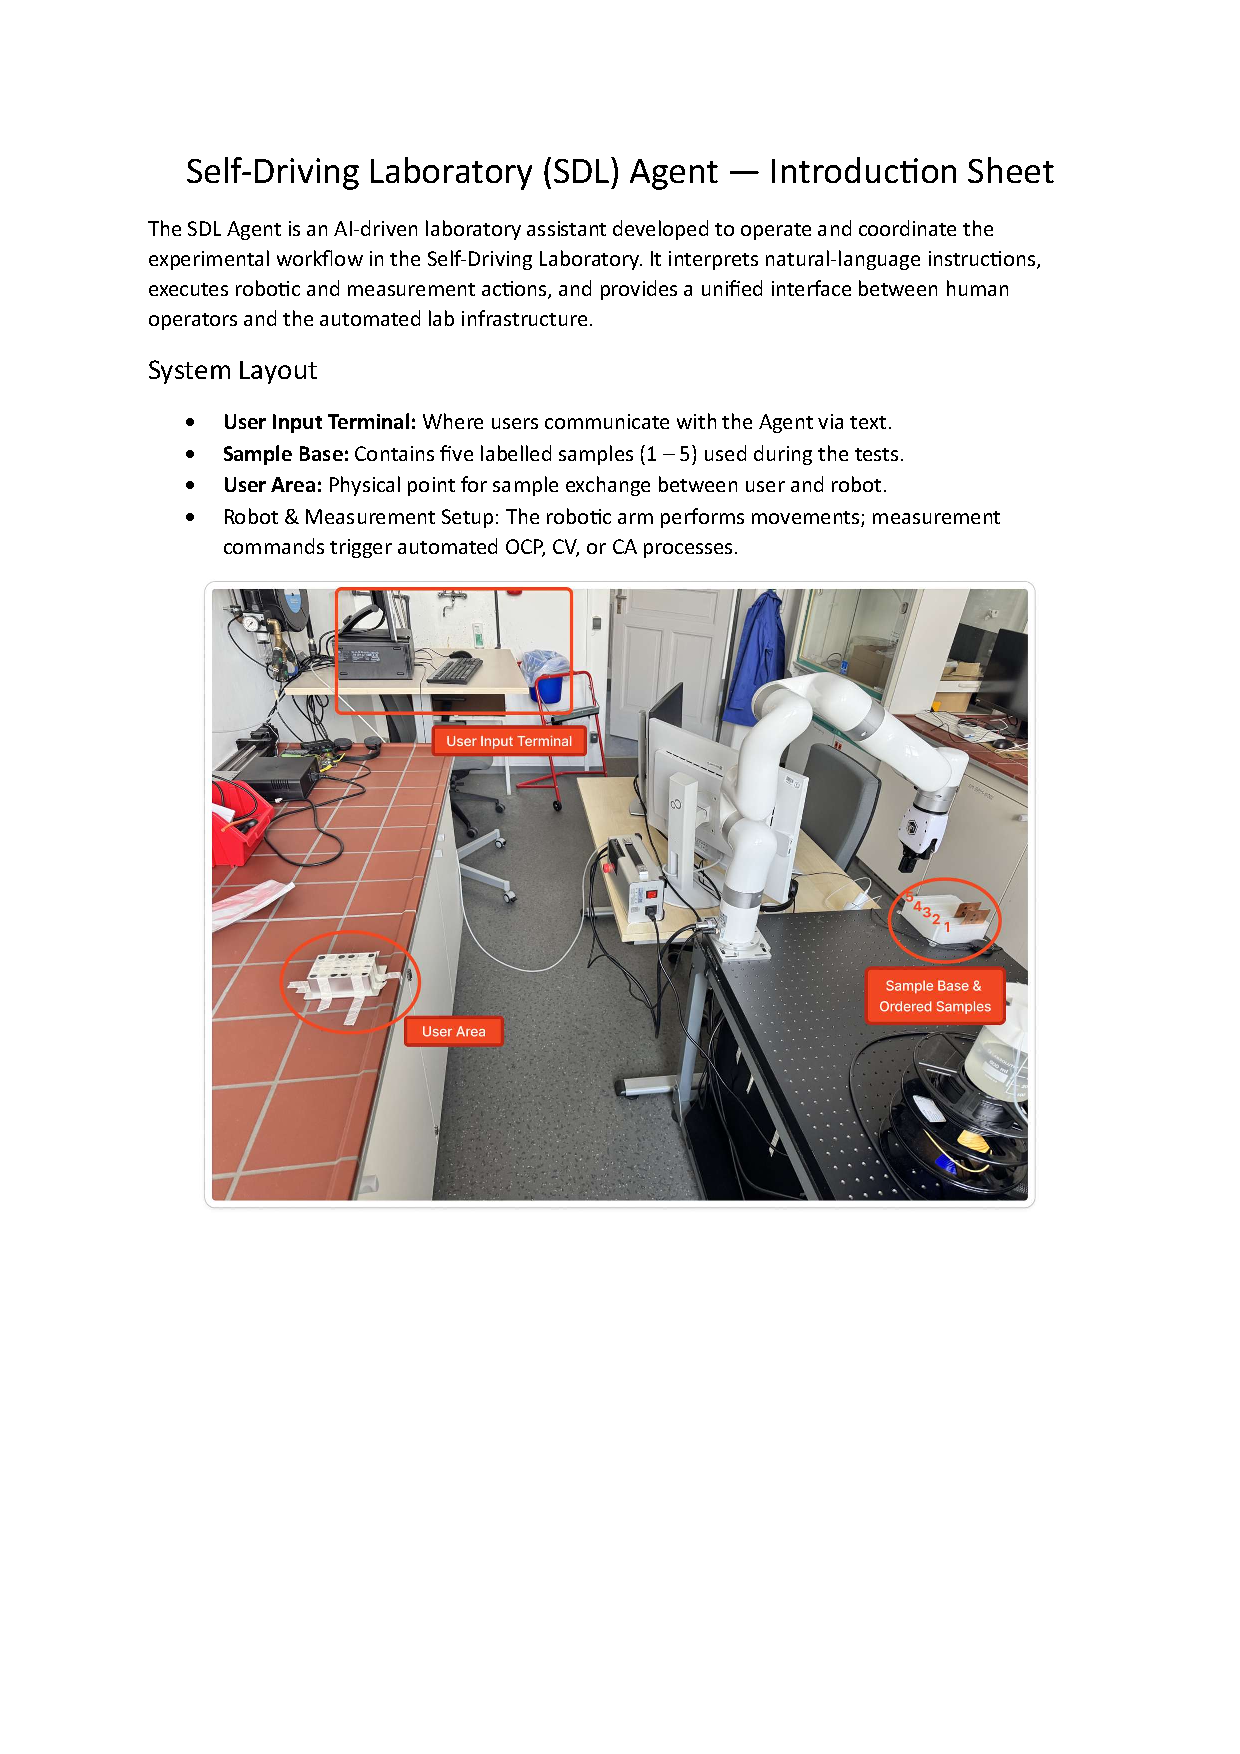
\includepdf{appendix/userguide.pdf}
}
\newpage
\ch{Codes}{codes}
The following listing shows the main section of the \texttt{labagent.py} used for initializing the SDL Agent.

\begin{lstlisting}[language=Python, caption={sdlagent.py}]
# labagent.py

from smolagents import CodeAgent, LiteLLMModel, GradioUI, tool
import toolsfake


@tool
def ocp_measurement(i: int) -> str:
    """
    Perform an OCP measurement on a given sample.

    Args:
        i (int): The sample index to measure.
    """
    result = toolsfake.ocp_measurement(i)   # prints
    return f"OCP measurement called for sample {i}"


@tool
def ca_measurement(i: int) -> str:
    """
    Perform a Chronoamperometry (CA) measurement on a given sample.

    Args:
        i (int): The sample index to measure.
    """
    result = toolsfake.ca_measurement(i)   # prints
    return f"CA measurement called for sample {i}"


@tool
def cv_measurement(i: int) -> str:
    """
    Perform a Cyclic Voltammetry (CV) measurement on a given sample.

    Args:
        i (int): The sample index to measure.
    """
    result = toolsfake.cv_measurement(i)   # prints
    return f"CV measurement called for sample {i}"


@tool
def bring_sample_to_user(i: int) -> str:
    """
    Bring a sample to the user.

    Args:
        i (int): The sample index to bring.
    """
    result = toolsfake.bring_sample_to_user(i)   # prints
    return f"Sample {i} brought to user"


@tool
def collect_sample_from_user(i: int) -> str:
    """
    Collect a sample from the user.

    Args:
        i (int): The sample index to collect.
    """
    result = toolsfake.collect_sample_from_user(i)   # prints
    return f"Sample {i} collected from user"


@tool
def go_home() -> str:
    """
    Send the robot to its home position.
    """
    result = toolsfake.go_home()   # prints
    return "Robot returned home"


model = LiteLLMModel(
    model_id="ollama/qwen2.5:7b-instruct",
    api_base="http://localhost:11434",
    system_prompt="You are a robotic lab assistant. Use ONLY the provided tools."
)


prompt = """
You are a laboratory robotic assistant.  
Your job is to directly execute the correct tool calls for the user’s request.  

RULES:
1. You may ONLY use the following tools:
   - ocp_measurement(i: int)
   - ca_measurement(i: int)
   - cv_measurement(i: int)
   - bring_sample_to_user(i: int)
   - collect_sample_from_user(i: int)
   - go_home()

2. Mapping rules:
   - "OCP" / "open circuit" / "potential" / "measure ocp" ⇒ ocp_measurement(i=...)
   - "CV" / "cyclic voltammetry" ⇒ cv_measurement(i=...)
   - "CA" / "chronoamperometry" / "chrono" ⇒ ca_measurement(i=...)
   - "bring/give/hand/pass/deliver TO me/user/operator" ⇒ bring_sample_to_user(i=...)
   - "take/get/receive/collect FROM me/user/hand/user area" ⇒ collect_sample_from_user(i=...)
   - "home/reset/base/park" ⇒ go_home()

3. Argument rules:
   - All tools except go_home require argument "i" (sample index).
   - Sample indices are integers in [1,5].
   - Interpret ordinals/cardinals: "first"=1, "second"=2, "third"=3, etc.
   - Accept ranges ("1-3", "1..3") or lists ("1 and 2", "1,2").
   - "all samples" ⇒ loop over [1,2,3,4,5].
   - If a later step omits the sample but clearly refers to the last one, reuse the last i.

4. Sequencing rules:
   - Parse connectors like "then", "after", "and".
   - Call the tools in order, one after another.

5. Output format:
   - Every answer must have exactly one `Thought:` line.
   - Then a `<code>...</code>` block with Python code.
   - Inside the code, call the tools step by step.
   - Always end with `final_answer("Done")` after executing the last step.
   - No JSON, no prose, no explanations outside the code.

EXAMPLES:

Q: do ocp for sample 1 then cv for sample 1  
A:
Thought: I need to run OCP for sample 1 and then CV for sample 1
<code>
ocp_measurement(i=1)
cv_measurement(i=1)
final_answer("Done")
</code>

Q: bring me the 5th, then go home  
A:
Thought: I need to bring sample 5 to the user and then send the robot home
<code>
bring_sample_to_user(i=5)
go_home()
final_answer("Done")
</code>

Q: do ocp for the 1st and 2nd sample then do cv for the 1st sample and ca for the 3rd  
A:
Thought: I need to run OCP for samples 1 and 2, then CV for sample 1, and CA for sample 3
<code>
ocp_measurement(i=1)
ocp_measurement(i=2)
cv_measurement(i=1)
ca_measurement(i=3)
final_answer("Done")
</code>

Q: do ocp for all samples then go home  
A:
Thought: I need to run OCP for all samples, then send the robot home
<code>
for i in [1,2,3,4,5]:
    ocp_measurement(i=i)
go_home()
final_answer("Done")
</code>
"""

agent = CodeAgent(
    model=model,
    tools=[ocp_measurement, ca_measurement, cv_measurement,
           bring_sample_to_user, collect_sample_from_user, go_home],
    instructions=prompt,
    add_base_tools=False
)


GradioUI(agent).launch()
\end{lstlisting}

The \texttt{tools.py} module defines the callable functions that form the interface between the AI Agent and the SDL hardware.  
Only the main functions are shown below for brevity; the complete version is archived in the digital supplement.

\begin{lstlisting}[language=Python, caption={tools.py}]
# tools.py

from instruments import *
from robotmotion import *
from store import *
from observation import *

def ocp_measurement(i: int) -> Observation:
    """
    Perform an Open Circuit Potential (OCP) measurement on a specified sample.

    The robotic system automates the process of measuring the OCP of a sample. 
    It picks up the sample from its starting slot, moves it to the measurement 
    station, interacts with the measurement device to analyze the sample, and 
    finally returns the sample to its original slot.

    Args:
        i (int): The index of the sample to measure.

    Returns:
        Observation: An object containing details of the measurement process, 
        including the measured value, duration, and metadata.

    Process:
        1. The robot picks up the sample from its designated slot on the bed.
        2. The sample is placed at the measurement station.
        3. The measurement device performs the OCP analysis and returns the result.
        4. The robot retrieves the sample from the measurement station.
        5. The sample is returned to its original slot on the bed.
        6. The observation is logged, including success or error details.

    Example:
        >>> obs = ocp_measurement(1)
        >>> print(obs.feature)
        OCP
        >>> print(obs.value)
        0.123  # Example measured value
    """
    obs = start_obs(step="measurement", tool="ocp_measurement", args={"i": i})
    try:
        uFactory_xArm.pick_sample_from_bed(i)
        uFactory_xArm.place_sample_to_measurementstation()
        f = "OCP"
        v = instruments.ocp_measurement_step()
        uFactory_xArm.pick_sample_from_measurementstation()
        uFactory_xArm.place_sample_to_bed(i)
        obs = finish_ok(obs, feature=f, sample=i, value=v, extra_meta={"pose": "measurementstation"})
    except Exception as e:
        obs = finish_err(obs, e)
    finally:
        log_observation(obs)
    return obs

def ca_measurement(i: int) -> Observation:
    """
    Perform a Chronoamperometry (CA) measurement on a specified sample.

    The robotic system automates the process of measuring the CA of a sample. 
    It picks up the sample from its starting slot, moves it to the measurement 
    station, interacts with the measurement device to analyze the sample, and 
    finally returns the sample to its original slot.

    Args:
        i (int): The index of the sample to measure.

    Returns:
        Observation: An object containing details of the measurement process, 
        including the measured value, duration, and metadata.

    Process:
        1. The robot picks up the sample from its designated slot on the bed.
        2. The sample is placed at the measurement station.
        3. The measurement device performs the CA analysis and returns the result.
        4. The robot retrieves the sample from the measurement station.
        5. The sample is returned to its original slot on the bed.
        6. The observation is logged, including success or error details.

    Example:
        >>> obs = ca_measurement(2)
        >>> print(obs.feature)
        CA
        >>> print(obs.value)
        0.456  # Example measured value
    """    
    obs = start_obs(step="measurement", tool="ca_measurement", args={"i": i})
    try:
        uFactory_xArm.pick_sample_from_bed(i)
        uFactory_xArm.place_sample_to_measurementstation()
        f="CA"
        v = instruments.ca_measurement_step()
        uFactory_xArm.pick_sample_from_measurementstation()
        uFactory_xArm.place_sample_to_bed(i)
        obs = finish_ok(obs,feature=f, sample=i, value=v, extra_meta={"pose": "measurementstation"})
    except Exception as e:
        obs = finish_err(obs, e)
    finally:
        log_observation(obs)
    return obs

def cv_measurement(i: int) -> Observation:
    """
    Perform a Cyclic Voltammetry (CV) measurement on a specified sample.

    The robotic system automates the process of measuring the CV of a sample. 
    It picks up the sample from its starting slot, moves it to the measurement 
    station, interacts with the measurement device to analyze the sample, and 
    finally returns the sample to its original slot.

    Args:
        i (int): The index of the sample to measure.

    Returns:
        Observation: An object containing details of the measurement process, 
        including the measured value, duration, and metadata.

    Process:
        1. The robot picks up the sample from its designated slot on the bed.
        2. The sample is placed at the measurement station.
        3. The measurement device performs the CV analysis and returns the result.
        4. The robot retrieves the sample from the measurement station.
        5. The sample is returned to its original slot on the bed.
        6. The observation is logged, including success or error details.

    Example:
        >>> obs = cv_measurement(3)
        >>> print(obs.feature)
        CV
        >>> print(obs.value)
        0.789  # Example measured value
    """
    obs = start_obs(step="measurement", tool="cv_measurement", args={"i": i})
    try:
        uFactory_xArm.pick_sample_from_bed(i)
        uFactory_xArm.place_sample_to_measurementstation()
        f="CV"
        v = instruments.cv_measurement_step()
        uFactory_xArm.pick_sample_from_measurementstation()
        uFactory_xArm.place_sample_to_bed(i)
        obs = finish_ok(obs, feature=f, sample=i, value=v, extra_meta={"pose": "measurementstation"})
    except Exception as e:
        obs = finish_err(obs, e)
    finally:
        log_observation(obs)
    return obs

def bring_sample_to_user(i: int) -> Observation:
    """
    Bring a specified sample to the user area.

    The robotic system picks up the sample from its designated slot on the bed 
    and places it in the user area for interaction.

    Args:
        i (int): The index of the sample to bring to the user.

    Returns:
        Observation: An object containing details of the operation, including 
        the sample index, duration, and metadata.

    Process:
        1. The robot picks up the sample from its designated slot on the bed.
        2. The sample is placed in the user area.
        3. The observation is logged, including success or error details.

    Example:
        >>> obs = bring_sample_to_user(4)
        >>> print(obs.meta["target"])
        userarea
    """
    obs = start_obs(step="interraction", tool="bring_sample_to_user", args={"i": i})
    try:
        uFactory_xArm.pick_sample_from_bed(i)
        uFactory_xArm.place_sample_to_userarea()
        obs = finish_ok(obs, sample=i, extra_meta={"target": "userarea"})
    except Exception as e:
        obs = finish_err(obs, e)
    finally:
        log_observation(obs)
    return obs

def collect_sample_from_user(i: int) -> Observation:
    """
    Collect a specified sample from the user area and return it to its original slot.

    The robotic system picks up the sample from the user area and places it back 
    in its designated slot on the bed.

    Args:
        i (int): The index of the sample to collect from the user.

    Returns:
        Observation: An object containing details of the operation, including 
        the sample index, duration, and metadata.

    Process:
        1. The robot picks up the sample from the user area.
        2. The sample is returned to its designated slot on the bed.
        3. The observation is logged, including success or error details.

    Example:
        >>> obs = collect_sample_from_user(5)
        >>> print(obs.meta["source"])
        userarea
    """
    obs = start_obs(step="interraction", tool="collect_sample_from_user", args={"i": i})
    try:
        uFactory_xArm.pick_sample_from_userarea()
        uFactory_xArm.place_sample_to_bed(i)
        obs = finish_ok(obs, sample=i, extra_meta={"source": "userarea"})
    except Exception as e:
        obs = finish_err(obs, e)
    finally:
        log_observation(obs)
    return obs

def go_home() -> Observation:
    """
    Move the robotic arm to its home position.

    The robotic system moves to its predefined home position, ensuring it is 
    in a safe and idle state.

    Returns:
        Observation: An object containing details of the operation, including 
        the duration and metadata.

    Process:
        1. The robot moves to its home position.
        2. The observation is logged, including success or error details.

    Example:
        >>> obs = go_home()
        >>> print(obs.meta["pose"])
        home
    """
    obs = start_obs(step="home", tool="go_home", args={})
    try:
        uFactory_xArm.move_to(uFactory_xArm.home)
        obs = finish_ok(obs, extra_meta={"pose": "home"})
    except Exception as e:
        obs = finish_err(obs, e)
    finally:
        log_observation(obs)
    return obs
\end{lstlisting}
\newpage
\ch{Experiemnts \& Queries}{experiments}

An excerpt from the generated JSONL result files used during simulation and real-user validation runs:

\begin{lstlisting}[language=json, caption={First 50 Simulated Queries}]
{"id": 1, "text": "do ocp for sample 1 then cv for sample 1", "smol_status": "success", "smol_time": 69.6959, "smol_trace": "OCP1CV1", "smol_inputtokens": 2048, "smol_outputtokens": 44}
{"id": 2, "text": "bring me the 5th, then go home", "smol_status": "success", "smol_time": 64.713, "smol_trace": "B5H", "smol_inputtokens": 2048, "smol_outputtokens": 41}
{"id": 3, "text": "do ca for sample 2 then bring me the 3rd", "smol_status": "success", "smol_time": 67.161, "smol_trace": "CA2B3", "smol_inputtokens": 2048, "smol_outputtokens": 47}
{"id": 4, "text": "do cv for the 4th sample and then go home", "smol_status": "success", "smol_time": 68.9077, "smol_trace": "CV4H", "smol_inputtokens": 2048, "smol_outputtokens": 38}
{"id": 5, "text": "bring me the 1st sample, then do ocp for it", "smol_status": "success", "smol_time": 73.6863, "smol_trace": "B1OCP1", "smol_inputtokens": 2048, "smol_outputtokens": 48}
{"id": 6, "text": "do ocp for all samples", "smol_status": "success", "smol_time": 66.2694, "smol_trace": "OCP1OCP2OCP3OCP4OCP5", "smol_inputtokens": 2048, "smol_outputtokens": 48}
{"id": 7, "text": "bring me the 2nd sample, then collect it back", "smol_status": "success", "smol_time": 66.2724, "smol_trace": "B2C2", "smol_inputtokens": 2048, "smol_outputtokens": 47}
{"id": 8, "text": "do ca for the 5th sample, then do cv for the 5th sample", "smol_status": "success", "smol_time": 68.1915, "smol_trace": "CA5CV5", "smol_inputtokens": 2048, "smol_outputtokens": 46}
{"id": 9, "text": "bring me the 4th sample, then go home", "smol_status": "success", "smol_time": 67.4166, "smol_trace": "B4H", "smol_inputtokens": 2048, "smol_outputtokens": 41}
{"id": 10, "text": "do ocp for the 3rd sample, then do ca for the 3rd sample", "smol_status": "success", "smol_time": 64.4669, "smol_trace": "OCP3CA3", "smol_inputtokens": 2048, "smol_outputtokens": 48}
{"id": 11, "text": "collect the 2nd sample from me, then do cv for it", "smol_status": "success", "smol_time": 69.2248, "smol_trace": "C2CV2", "smol_inputtokens": 2048, "smol_outputtokens": 47}
{"id": 12, "text": "do ocp for the 1st sample, then do cv for the 2nd sample", "smol_status": "success", "smol_time": 70.3344, "smol_trace": "OCP1CV2", "smol_inputtokens": 2048, "smol_outputtokens": 44}
{"id": 13, "text": "bring me the 5th sample, then do ca for it", "smol_status": "success", "smol_time": 69.2614, "smol_trace": "B5CA5", "smol_inputtokens": 2048, "smol_outputtokens": 45}
{"id": 14, "text": "do cv for the 3rd sample, then bring it to me", "smol_status": "success", "smol_time": 67.932, "smol_trace": "CV3B3", "smol_inputtokens": 2048, "smol_outputtokens": 44}
{"id": 15, "text": "do ocp for the 4th sample, then do ca for the 4th sample", "smol_status": "success", "smol_time": 73.652, "smol_trace": "OCP4CA4", "smol_inputtokens": 2048, "smol_outputtokens": 46}
{"id": 16, "text": "bring me the 2nd sample, then do cv for it", "smol_status": "success", "smol_time": 75.6158, "smol_trace": "B2CV2", "smol_inputtokens": 2048, "smol_outputtokens": 47}
{"id": 17, "text": "do ocp for the 1st and 2nd samples", "smol_status": "success", "smol_time": 73.2591, "smol_trace": "OCP1OCP2", "smol_inputtokens": 2048, "smol_outputtokens": 41}
{"id": 18, "text": "do ca for the 3rd sample, then go home", "smol_status": "success", "smol_time": 70.7498, "smol_trace": "CA3H", "smol_inputtokens": 2048, "smol_outputtokens": 38}
{"id": 19, "text": "bring me the 1st sample, then do ocp for it", "smol_status": "success", "smol_time": 70.9843, "smol_trace": "B1OCP1", "smol_inputtokens": 2048, "smol_outputtokens": 48}
{"id": 20, "text": "do cv for the 5th sample, then bring it to me", "smol_status": "success", "smol_time": 70.7262, "smol_trace": "CV5B5", "smol_inputtokens": 2048, "smol_outputtokens": 47}
{"id": 21, "text": "do ocp for the 2nd sample, then do ca for the 2nd sample", "smol_status": "success", "smol_time": 64.0255, "smol_trace": "OCP2CA2", "smol_inputtokens": 2048, "smol_outputtokens": 46}
{"id": 22, "text": "bring me the 3rd sample, then collect it back", "smol_status": "success", "smol_time": 62.7716, "smol_trace": "B3C3", "smol_inputtokens": 2048, "smol_outputtokens": 47}
{"id": 23, "text": "do ocp for the 4th sample, then do cv for the 4th sample", "smol_status": "success", "smol_time": 62.7042, "smol_trace": "OCP4CV4", "smol_inputtokens": 2048, "smol_outputtokens": 46}
{"id": 24, "text": "bring me the 5th sample, then do ocp for it", "smol_status": "success", "smol_time": 63.4909, "smol_trace": "B5OCP5", "smol_inputtokens": 2048, "smol_outputtokens": 48}
{"id": 25, "text": "do ca for the 1st sample, then bring it to me", "smol_status": "success", "smol_time": 62.5872, "smol_trace": "CA1B1", "smol_inputtokens": 2048, "smol_outputtokens": 45}
{"id": 26, "text": "do cv for the 2nd sample, then go home", "smol_status": "success", "smol_time": 61.7514, "smol_trace": "CV2H", "smol_inputtokens": 2048, "smol_outputtokens": 38}
{"id": 27, "text": "bring me the 4th sample, then do ca for it", "smol_status": "success", "smol_time": 63.7444, "smol_trace": "B4CA4", "smol_inputtokens": 2048, "smol_outputtokens": 51}
{"id": 28, "text": "do ocp for the 3rd sample, then do ca for the 3rd sample", "smol_status": "success", "smol_time": 62.9925, "smol_trace": "OCP3CA3", "smol_inputtokens": 2048, "smol_outputtokens": 48}
{"id": 29, "text": "collect the 1st sample from me, then do cv for it", "smol_status": "success", "smol_time": 62.4828, "smol_trace": "C1CV1", "smol_inputtokens": 2048, "smol_outputtokens": 45}
{"id": 30, "text": "do ocp for the 5th sample, then do cv for the 5th sample", "smol_status": "success", "smol_time": 62.269, "smol_trace": "OCP5CV5", "smol_inputtokens": 2048, "smol_outputtokens": 41}
{"id": 31, "text": "bring me the 2nd sample, then do ocp for it", "smol_status": "success", "smol_time": 63.1419, "smol_trace": "B2OCP2", "smol_inputtokens": 2048, "smol_outputtokens": 48}
{"id": 32, "text": "do ca for the 4th sample, then bring it to me", "smol_status": "success", "smol_time": 62.7005, "smol_trace": "CA4B4", "smol_inputtokens": 2048, "smol_outputtokens": 47}
{"id": 33, "text": "do cv for the 1st sample, then go home", "smol_status": "success", "smol_time": 62.4952, "smol_trace": "CV1H", "smol_inputtokens": 2048, "smol_outputtokens": 38}
{"id": 34, "text": "bring me the 3rd sample, then do ca for it", "smol_status": "success", "smol_time": 63.1172, "smol_trace": "B3CA3", "smol_inputtokens": 2048, "smol_outputtokens": 45}
{"id": 35, "text": "do ocp for the 2nd sample, then do ca for the 2nd sample", "smol_status": "success", "smol_time": 63.536, "smol_trace": "OCP2CA2", "smol_inputtokens": 2048, "smol_outputtokens": 44}
{"id": 36, "text": "bring me the 5th sample, then collect it back", "smol_status": "success", "smol_time": 63.8274, "smol_trace": "B5C5", "smol_inputtokens": 2048, "smol_outputtokens": 45}
{"id": 37, "text": "do ocp for the 4th sample, then do cv for the 4th sample", "smol_status": "success", "smol_time": 64.3786, "smol_trace": "OCP4CV4", "smol_inputtokens": 2048, "smol_outputtokens": 48}
{"id": 38, "text": "bring me the 1st sample, then do ocp for it", "smol_status": "success", "smol_time": 67.3458, "smol_trace": "B1OCP1", "smol_inputtokens": 2048, "smol_outputtokens": 48}
{"id": 39, "text": "do ca for the 3rd sample, then bring it to me", "smol_status": "success", "smol_time": 70.8254, "smol_trace": "CA3B3", "smol_inputtokens": 2048, "smol_outputtokens": 47}
{"id": 40, "text": "do cv for the 2nd sample, then go home", "smol_status": "success", "smol_time": 64.8269, "smol_trace": "CV2H", "smol_inputtokens": 2048, "smol_outputtokens": 38}
{"id": 41, "text": "bring me the 4th sample, then do ca for it", "smol_status": "success", "smol_time": 64.5768, "smol_trace": "B4CA4", "smol_inputtokens": 2048, "smol_outputtokens": 47}
{"id": 42, "text": "do ocp for the 5th sample, then do ca for the 5th sample", "smol_status": "success", "smol_time": 65.2011, "smol_trace": "OCP5CA5", "smol_inputtokens": 2048, "smol_outputtokens": 44}
{"id": 43, "text": "collect the 3rd sample from me, then do cv for it", "smol_status": "success", "smol_time": 65.1564, "smol_trace": "C3CV3", "smol_inputtokens": 2048, "smol_outputtokens": 47}
{"id": 44, "text": "do ocp for the 1st sample, then do cv for the 1st sample", "smol_status": "success", "smol_time": 66.7488, "smol_trace": "OCP1CV1", "smol_inputtokens": 2048, "smol_outputtokens": 44}
{"id": 45, "text": "bring me the 2nd sample, then do ocp for it", "smol_status": "success", "smol_time": 66.6776, "smol_trace": "B2OCP2", "smol_inputtokens": 2048, "smol_outputtokens": 50}
{"id": 46, "text": "do ca for the 4th sample, then bring it to me", "smol_status": "success", "smol_time": 67.9285, "smol_trace": "CA4B4", "smol_inputtokens": 2048, "smol_outputtokens": 44}
{"id": 47, "text": "do cv for the 5th sample, then go home", "smol_status": "success", "smol_time": 65.4711, "smol_trace": "CV5H", "smol_inputtokens": 2048, "smol_outputtokens": 38}
{"id": 48, "text": "bring me the 3rd sample, then do ca for it", "smol_status": "success", "smol_time": 68.4682, "smol_trace": "B3CA3", "smol_inputtokens": 2048, "smol_outputtokens": 47}
{"id": 49, "text": "do ocp for the 2nd sample, then do ca for the 2nd sample", "smol_status": "success", "smol_time": 66.727, "smol_trace": "OCP2CA2", "smol_inputtokens": 2048, "smol_outputtokens": 44}
{"id": 50, "text": "bring me the 1st sample, then collect it back", "smol_status": "success", "smol_time": 67.4304, "smol_trace": "B1C1", "smol_inputtokens": 2048, "smol_outputtokens": 45}
\end{lstlisting}

\begin{lstlisting}[language=json, caption={Additional 100 Simulated Queries}]
{"id": 1, "text": "do ocp for sample 1 then cv for sample 1", "smol_status": "success", "smol_time": 69.6959, "smol_trace": "OCP1CV1", "smol_inputtokens": 2048, "smol_outputtokens": 44}
{"id": 2, "text": "bring me the 5th, then go home", "smol_status": "success", "smol_time": 64.713, "smol_trace": "B5H", "smol_inputtokens": 2048, "smol_outputtokens": 41}
{"id": 3, "text": "do ca for sample 2 then bring me the 3rd", "smol_status": "success", "smol_time": 67.161, "smol_trace": "CA2B3", "smol_inputtokens": 2048, "smol_outputtokens": 47}
{"id": 4, "text": "do cv for the 4th sample and then go home", "smol_status": "success", "smol_time": 68.9077, "smol_trace": "CV4H", "smol_inputtokens": 2048, "smol_outputtokens": 38}
{"id": 5, "text": "bring me the 1st sample, then do ocp for it", "smol_status": "success", "smol_time": 73.6863, "smol_trace": "B1OCP1", "smol_inputtokens": 2048, "smol_outputtokens": 48}
{"id": 6, "text": "do ocp for all samples", "smol_status": "success", "smol_time": 66.2694, "smol_trace": "OCP1OCP2OCP3OCP4OCP5", "smol_inputtokens": 2048, "smol_outputtokens": 48}
{"id": 7, "text": "bring me the 2nd sample, then collect it back", "smol_status": "success", "smol_time": 66.2724, "smol_trace": "B2C2", "smol_inputtokens": 2048, "smol_outputtokens": 47}
{"id": 8, "text": "do ca for the 5th sample, then do cv for the 5th sample", "smol_status": "success", "smol_time": 68.1915, "smol_trace": "CA5CV5", "smol_inputtokens": 2048, "smol_outputtokens": 46}
{"id": 9, "text": "bring me the 4th sample, then go home", "smol_status": "success", "smol_time": 67.4166, "smol_trace": "B4H", "smol_inputtokens": 2048, "smol_outputtokens": 41}
{"id": 10, "text": "do ocp for the 3rd sample, then do ca for the 3rd sample", "smol_status": "success", "smol_time": 64.4669, "smol_trace": "OCP3CA3", "smol_inputtokens": 2048, "smol_outputtokens": 48}
{"id": 11, "text": "collect the 2nd sample from me, then do cv for it", "smol_status": "success", "smol_time": 69.2248, "smol_trace": "C2CV2", "smol_inputtokens": 2048, "smol_outputtokens": 47}
{"id": 12, "text": "do ocp for the 1st sample, then do cv for the 2nd sample", "smol_status": "success", "smol_time": 70.3344, "smol_trace": "OCP1CV2", "smol_inputtokens": 2048, "smol_outputtokens": 44}
{"id": 13, "text": "bring me the 5th sample, then do ca for it", "smol_status": "success", "smol_time": 69.2614, "smol_trace": "B5CA5", "smol_inputtokens": 2048, "smol_outputtokens": 45}
{"id": 14, "text": "do cv for the 3rd sample, then bring it to me", "smol_status": "success", "smol_time": 67.932, "smol_trace": "CV3B3", "smol_inputtokens": 2048, "smol_outputtokens": 44}
{"id": 15, "text": "do ocp for the 4th sample, then do ca for the 4th sample", "smol_status": "success", "smol_time": 73.652, "smol_trace": "OCP4CA4", "smol_inputtokens": 2048, "smol_outputtokens": 46}
{"id": 16, "text": "bring me the 2nd sample, then do cv for it", "smol_status": "success", "smol_time": 75.6158, "smol_trace": "B2CV2", "smol_inputtokens": 2048, "smol_outputtokens": 47}
{"id": 17, "text": "do ocp for the 1st and 2nd samples", "smol_status": "success", "smol_time": 73.2591, "smol_trace": "OCP1OCP2", "smol_inputtokens": 2048, "smol_outputtokens": 41}
{"id": 18, "text": "do ca for the 3rd sample, then go home", "smol_status": "success", "smol_time": 70.7498, "smol_trace": "CA3H", "smol_inputtokens": 2048, "smol_outputtokens": 38}
{"id": 19, "text": "bring me the 1st sample, then do ocp for it", "smol_status": "success", "smol_time": 70.9843, "smol_trace": "B1OCP1", "smol_inputtokens": 2048, "smol_outputtokens": 48}
{"id": 20, "text": "do cv for the 5th sample, then bring it to me", "smol_status": "success", "smol_time": 70.7262, "smol_trace": "CV5B5", "smol_inputtokens": 2048, "smol_outputtokens": 47}
{"id": 21, "text": "do ocp for the 2nd sample, then do ca for the 2nd sample", "smol_status": "success", "smol_time": 64.0255, "smol_trace": "OCP2CA2", "smol_inputtokens": 2048, "smol_outputtokens": 46}
{"id": 22, "text": "bring me the 3rd sample, then collect it back", "smol_status": "success", "smol_time": 62.7716, "smol_trace": "B3C3", "smol_inputtokens": 2048, "smol_outputtokens": 47}
{"id": 23, "text": "do ocp for the 4th sample, then do cv for the 4th sample", "smol_status": "success", "smol_time": 62.7042, "smol_trace": "OCP4CV4", "smol_inputtokens": 2048, "smol_outputtokens": 46}
{"id": 24, "text": "bring me the 5th sample, then do ocp for it", "smol_status": "success", "smol_time": 63.4909, "smol_trace": "B5OCP5", "smol_inputtokens": 2048, "smol_outputtokens": 48}
{"id": 25, "text": "do ca for the 1st sample, then bring it to me", "smol_status": "success", "smol_time": 62.5872, "smol_trace": "CA1B1", "smol_inputtokens": 2048, "smol_outputtokens": 45}
{"id": 26, "text": "do cv for the 2nd sample, then go home", "smol_status": "success", "smol_time": 61.7514, "smol_trace": "CV2H", "smol_inputtokens": 2048, "smol_outputtokens": 38}
{"id": 27, "text": "bring me the 4th sample, then do ca for it", "smol_status": "success", "smol_time": 63.7444, "smol_trace": "B4CA4", "smol_inputtokens": 2048, "smol_outputtokens": 51}
{"id": 28, "text": "do ocp for the 3rd sample, then do ca for the 3rd sample", "smol_status": "success", "smol_time": 62.9925, "smol_trace": "OCP3CA3", "smol_inputtokens": 2048, "smol_outputtokens": 48}
{"id": 29, "text": "collect the 1st sample from me, then do cv for it", "smol_status": "success", "smol_time": 62.4828, "smol_trace": "C1CV1", "smol_inputtokens": 2048, "smol_outputtokens": 45}
{"id": 30, "text": "do ocp for the 5th sample, then do cv for the 5th sample", "smol_status": "success", "smol_time": 62.269, "smol_trace": "OCP5CV5", "smol_inputtokens": 2048, "smol_outputtokens": 41}
{"id": 31, "text": "bring me the 2nd sample, then do ocp for it", "smol_status": "success", "smol_time": 63.1419, "smol_trace": "B2OCP2", "smol_inputtokens": 2048, "smol_outputtokens": 48}
{"id": 32, "text": "do ca for the 4th sample, then bring it to me", "smol_status": "success", "smol_time": 62.7005, "smol_trace": "CA4B4", "smol_inputtokens": 2048, "smol_outputtokens": 47}
{"id": 33, "text": "do cv for the 1st sample, then go home", "smol_status": "success", "smol_time": 62.4952, "smol_trace": "CV1H", "smol_inputtokens": 2048, "smol_outputtokens": 38}
{"id": 34, "text": "bring me the 3rd sample, then do ca for it", "smol_status": "success", "smol_time": 63.1172, "smol_trace": "B3CA3", "smol_inputtokens": 2048, "smol_outputtokens": 45}
{"id": 35, "text": "do ocp for the 2nd sample, then do ca for the 2nd sample", "smol_status": "success", "smol_time": 63.536, "smol_trace": "OCP2CA2", "smol_inputtokens": 2048, "smol_outputtokens": 44}
{"id": 36, "text": "bring me the 5th sample, then collect it back", "smol_status": "success", "smol_time": 63.8274, "smol_trace": "B5C5", "smol_inputtokens": 2048, "smol_outputtokens": 45}
{"id": 37, "text": "do ocp for the 4th sample, then do cv for the 4th sample", "smol_status": "success", "smol_time": 64.3786, "smol_trace": "OCP4CV4", "smol_inputtokens": 2048, "smol_outputtokens": 48}
{"id": 38, "text": "bring me the 1st sample, then do ocp for it", "smol_status": "success", "smol_time": 67.3458, "smol_trace": "B1OCP1", "smol_inputtokens": 2048, "smol_outputtokens": 48}
{"id": 39, "text": "do ca for the 3rd sample, then bring it to me", "smol_status": "success", "smol_time": 70.8254, "smol_trace": "CA3B3", "smol_inputtokens": 2048, "smol_outputtokens": 47}
{"id": 40, "text": "do cv for the 2nd sample, then go home", "smol_status": "success", "smol_time": 64.8269, "smol_trace": "CV2H", "smol_inputtokens": 2048, "smol_outputtokens": 38}
{"id": 41, "text": "bring me the 4th sample, then do ca for it", "smol_status": "success", "smol_time": 64.5768, "smol_trace": "B4CA4", "smol_inputtokens": 2048, "smol_outputtokens": 47}
{"id": 42, "text": "do ocp for the 5th sample, then do ca for the 5th sample", "smol_status": "success", "smol_time": 65.2011, "smol_trace": "OCP5CA5", "smol_inputtokens": 2048, "smol_outputtokens": 44}
{"id": 43, "text": "collect the 3rd sample from me, then do cv for it", "smol_status": "success", "smol_time": 65.1564, "smol_trace": "C3CV3", "smol_inputtokens": 2048, "smol_outputtokens": 47}
{"id": 44, "text": "do ocp for the 1st sample, then do cv for the 1st sample", "smol_status": "success", "smol_time": 66.7488, "smol_trace": "OCP1CV1", "smol_inputtokens": 2048, "smol_outputtokens": 44}
{"id": 45, "text": "bring me the 2nd sample, then do ocp for it", "smol_status": "success", "smol_time": 66.6776, "smol_trace": "B2OCP2", "smol_inputtokens": 2048, "smol_outputtokens": 50}
{"id": 46, "text": "do ca for the 4th sample, then bring it to me", "smol_status": "success", "smol_time": 67.9285, "smol_trace": "CA4B4", "smol_inputtokens": 2048, "smol_outputtokens": 44}
{"id": 47, "text": "do cv for the 5th sample, then go home", "smol_status": "success", "smol_time": 65.4711, "smol_trace": "CV5H", "smol_inputtokens": 2048, "smol_outputtokens": 38}
{"id": 48, "text": "bring me the 3rd sample, then do ca for it", "smol_status": "success", "smol_time": 68.4682, "smol_trace": "B3CA3", "smol_inputtokens": 2048, "smol_outputtokens": 47}
{"id": 49, "text": "do ocp for the 2nd sample, then do ca for the 2nd sample", "smol_status": "success", "smol_time": 66.727, "smol_trace": "OCP2CA2", "smol_inputtokens": 2048, "smol_outputtokens": 44}
{"id": 50, "text": "bring me the 1st sample, then collect it back", "smol_status": "success", "smol_time": 67.4304, "smol_trace": "B1C1", "smol_inputtokens": 2048, "smol_outputtokens": 45}
{"id": 1, "text": "do ocp for sample 1 then cv for sample 1", "smol_status": "success", "smol_time": 103.4814, "smol_trace": "OCP1CV1", "smol_inputtokens": 2048, "smol_outputtokens": 44}
{"id": 2, "text": "bring me the 5th, then go home", "smol_status": "success", "smol_time": 70.6626, "smol_trace": "B5H", "smol_inputtokens": 2048, "smol_outputtokens": 41}
{"id": 3, "text": "do ca for sample 2 then bring me the 3rd", "smol_status": "success", "smol_time": 71.5897, "smol_trace": "CA2B3", "smol_inputtokens": 2048, "smol_outputtokens": 47}
{"id": 4, "text": "do cv for the 4th sample and then go home", "smol_status": "success", "smol_time": 70.8355, "smol_trace": "CV4H", "smol_inputtokens": 2048, "smol_outputtokens": 38}
{"id": 5, "text": "please bring the first sample and afterwards measure its ocp", "smol_status": "success", "smol_time": 70.7577, "smol_trace": "B1OCP1", "smol_inputtokens": 2048, "smol_outputtokens": 45}
{"id": 6, "text": "perform ocp measurements sequentially on all samples", "smol_status": "success", "smol_time": 71.3525, "smol_trace": "OCP1OCP2OCP3OCP4OCP5", "smol_inputtokens": 2048, "smol_outputtokens": 50}
{"id": 7, "text": "fetch sample 2 to the user zone and put it back later", "smol_status": "success", "smol_time": 71.618, "smol_trace": "B2C2", "smol_inputtokens": 2048, "smol_outputtokens": 47}
{"id": 8, "text": "run chronoamperometry then cyclic voltammetry for sample 5", "smol_status": "success", "smol_time": 70.0491, "smol_trace": "CA5CV5", "smol_inputtokens": 2048, "smol_outputtokens": 42}
{"id": 9, "text": "retrieve the fourth specimen and park the arm home", "smol_status": "success", "smol_time": 70.4824, "smol_trace": "B4H", "smol_inputtokens": 2048, "smol_outputtokens": 43}
{"id": 10, "text": "conduct ocp then ca on the 3rd specimen", "smol_status": "success", "smol_time": 71.881, "smol_trace": "OCP3CA3", "smol_inputtokens": 2048, "smol_outputtokens": 48}
{"id": 11, "text": "collect sample 2 from user area and perform cv", "smol_status": "success", "smol_time": 70.5067, "smol_trace": "C2CV2", "smol_inputtokens": 2048, "smol_outputtokens": 45}
{"id": 12, "text": "do ocp for the first, then cv for the second sample", "smol_status": "success", "smol_time": 72.18, "smol_trace": "OCP1CV2", "smol_inputtokens": 2048, "smol_outputtokens": 44}
{"id": 13, "text": "grab the fifth sample and carry out ca", "smol_status": "success", "smol_time": 71.3409, "smol_trace": "B5CA5", "smol_inputtokens": 2048, "smol_outputtokens": 47}
{"id": 14, "text": "run cv for the third one and hand it to me", "smol_status": "success", "smol_time": 70.8013, "smol_trace": "CV3B3", "smol_inputtokens": 2048, "smol_outputtokens": 44}
{"id": 15, "text": "analyze sample four with ocp then ca", "smol_status": "success", "smol_time": 72.1218, "smol_trace": "OCP4CA4", "smol_inputtokens": 2048, "smol_outputtokens": 44}
{"id": 16, "text": "bring sample two first and execute cv afterwards", "smol_status": "success", "smol_time": 80.5473, "smol_trace": "B2CV2", "smol_inputtokens": 2048, "smol_outputtokens": 50}
{"id": 17, "text": "measure ocp for samples one and two", "smol_status": "success", "smol_time": 74.4176, "smol_trace": "OCP1OCP2", "smol_inputtokens": 2048, "smol_outputtokens": 42}
{"id": 18, "text": "perform ca on the third then go home", "smol_status": "success", "smol_time": 70.9724, "smol_trace": "CA3H", "smol_inputtokens": 2048, "smol_outputtokens": 39}
{"id": 19, "text": "fetch sample 1 and take its ocp reading", "smol_status": "success", "smol_time": 71.131, "smol_trace": "B1OCP1", "smol_inputtokens": 2048, "smol_outputtokens": 45}
{"id": 20, "text": "carry out cv for sample 5 and bring it here", "smol_status": "success", "smol_time": 70.9956, "smol_trace": "CV5B5", "smol_inputtokens": 2048, "smol_outputtokens": 46}
{"id": 21, "text": "execute ocp followed by ca for specimen 2", "smol_status": "success", "smol_time": 84.8935, "smol_trace": "OCP2CA2", "smol_inputtokens": 2048, "smol_outputtokens": 40}
{"id": 22, "text": "deliver the third sample and later collect it", "smol_status": "success", "smol_time": 91.7991, "smol_trace": "B3C3", "smol_inputtokens": 2048, "smol_outputtokens": 42}
{"id": 23, "text": "perform ocp then cv on sample four", "smol_status": "success", "smol_time": 91.4578, "smol_trace": "OCP4CV4", "smol_inputtokens": 2048, "smol_outputtokens": 44}
{"id": 24, "text": "get sample five, run ocp", "smol_status": "success", "smol_time": 90.3996, "smol_trace": "B5OCP5", "smol_inputtokens": 2048, "smol_outputtokens": 46}
{"id": 25, "text": "run ca on the first and then hand it to me", "smol_status": "success", "smol_time": 93.6813, "smol_trace": "CA1B1", "smol_inputtokens": 2048, "smol_outputtokens": 47}
{"id": 26, "text": "measure cv on second and park home", "smol_status": "success", "smol_time": 87.9694, "smol_trace": "CV2H", "smol_inputtokens": 2048, "smol_outputtokens": 38}
{"id": 27, "text": "bring fourth, then execute ca", "smol_status": "success", "smol_time": 91.7313, "smol_trace": "B4CA4", "smol_inputtokens": 2048, "smol_outputtokens": 47}
{"id": 28, "text": "conduct ocp then ca on number three", "smol_status": "success", "smol_time": 93.141, "smol_trace": "OCP3CA3", "smol_inputtokens": 2048, "smol_outputtokens": 40}
{"id": 29, "text": "take back sample one from user and do cv", "smol_status": "success", "smol_time": 91.2179, "smol_trace": "C1CV1", "smol_inputtokens": 2048, "smol_outputtokens": 45}
{"id": 30, "text": "perform ocp then cv on fifth sample", "smol_status": "success", "smol_time": 89.2704, "smol_trace": "OCP5CV5", "smol_inputtokens": 2048, "smol_outputtokens": 44}
{"id": 31, "text": "fetch second specimen then run ocp", "smol_status": "success", "smol_time": 90.7561, "smol_trace": "B2OCP2", "smol_inputtokens": 2048, "smol_outputtokens": 50}
{"id": 32, "text": "carry out ca for fourth and then bring it here", "smol_status": "success", "smol_time": 91.9755, "smol_trace": "CA4B4", "smol_inputtokens": 2048, "smol_outputtokens": 50}
{"id": 33, "text": "cv on first, finish by homing", "smol_status": "success", "smol_time": 91.2135, "smol_trace": "CV1H", "smol_inputtokens": 2048, "smol_outputtokens": 39}
{"id": 34, "text": "bring the third piece and perform ca", "smol_status": "success", "smol_time": 93.2746, "smol_trace": "B3CA3", "smol_inputtokens": 2048, "smol_outputtokens": 44}
{"id": 35, "text": "run ocp then ca for sample two", "smol_status": "success", "smol_time": 96.3182, "smol_trace": "OCP2CA2", "smol_inputtokens": 2048, "smol_outputtokens": 44}
{"id": 36, "text": "deliver fifth to me then return it", "smol_status": "success", "smol_time": 93.1156, "smol_trace": "B5C5", "smol_inputtokens": 2048, "smol_outputtokens": 49}
{"id": 37, "text": "ocp then cv for fourth", "smol_status": "success", "smol_time": 92.0593, "smol_trace": "OCP4CV4", "smol_inputtokens": 2048, "smol_outputtokens": 48}
{"id": 38, "text": "bring the first one and run ocp", "smol_status": "success", "smol_time": 91.67, "smol_trace": "B1OCP1", "smol_inputtokens": 2048, "smol_outputtokens": 48}
{"id": 39, "text": "do ca on the third then give it to user", "smol_status": "success", "smol_time": 92.1582, "smol_trace": "CA3B3", "smol_inputtokens": 2048, "smol_outputtokens": 45}
{"id": 40, "text": "cv measurement for sample two then home", "smol_status": "success", "smol_time": 91.754, "smol_trace": "CV2H", "smol_inputtokens": 2048, "smol_outputtokens": 39}
{"id": 41, "text": "retrieve fourth sample, perform ca", "smol_status": "success", "smol_time": 88.8974, "smol_trace": "B4CA4", "smol_inputtokens": 2048, "smol_outputtokens": 46}
{"id": 42, "text": "ocp then ca on sample five", "smol_status": "success", "smol_time": 83.3984, "smol_trace": "OCP5CA5", "smol_inputtokens": 2048, "smol_outputtokens": 42}
{"id": 43, "text": "pick third from user and do cv", "smol_status": "success", "smol_time": 83.8248, "smol_trace": "C3CV3", "smol_inputtokens": 2048, "smol_outputtokens": 44}
{"id": 44, "text": "run ocp and cv for sample one", "smol_status": "success", "smol_time": 83.9002, "smol_trace": "OCP1CV1", "smol_inputtokens": 2048, "smol_outputtokens": 39}
{"id": 45, "text": "fetch second sample then analyze ocp", "smol_status": "success", "smol_time": 87.5002, "smol_trace": "B2OCP2", "smol_inputtokens": 2048, "smol_outputtokens": 48}
{"id": 46, "text": "ca on fourth, bring it to me", "smol_status": "success", "smol_time": 84.472, "smol_trace": "CA4B4", "smol_inputtokens": 2048, "smol_outputtokens": 49}
{"id": 47, "text": "perform cv for sample five, then home", "smol_status": "success", "smol_time": 82.7002, "smol_trace": "CV5H", "smol_inputtokens": 2048, "smol_outputtokens": 39}
{"id": 48, "text": "bring third and execute ca", "smol_status": "success", "smol_time": 84.3757, "smol_trace": "B3CA3", "smol_inputtokens": 2048, "smol_outputtokens": 45}
{"id": 49, "text": "ocp then ca for second sample", "smol_status": "success", "smol_time": 85.5175, "smol_trace": "OCP2CA2", "smol_inputtokens": 2048, "smol_outputtokens": 44}
{"id": 50, "text": "retrieve first sample then collect", "smol_status": "success", "smol_time": 84.2102, "smol_trace": "B1C1", "smol_inputtokens": 2048, "smol_outputtokens": 44}
{"id": 51, "text": "carry out cv for first then ca for first", "smol_status": "success", "smol_time": 83.8673, "smol_trace": "CV1CA1", "smol_inputtokens": 2048, "smol_outputtokens": 42}
{"id": 52, "text": "bring me number 4 then run ocp", "smol_status": "success", "smol_time": 84.7319, "smol_trace": "B4OCP4", "smol_inputtokens": 2048, "smol_outputtokens": 46}
{"id": 53, "text": "run ocp for sample three, afterwards bring it", "smol_status": "success", "smol_time": 83.8138, "smol_trace": "OCP3B3", "smol_inputtokens": 2048, "smol_outputtokens": 46}
{"id": 54, "text": "measure ca for sample 1 then cv", "smol_status": "success", "smol_time": 84.1581, "smol_trace": "CA1CV1", "smol_inputtokens": 2048, "smol_outputtokens": 40}
{"id": 55, "text": "bring the fifth sample then home the robot", "smol_status": "success", "smol_time": 84.31, "smol_trace": "B5H", "smol_inputtokens": 2048, "smol_outputtokens": 41}
{"id": 56, "text": "run ocp and cv on all specimens sequentially", "smol_status": "success", "smol_time": 86.7144, "smol_trace": "OCP1CV1OCP2CV2OCP3CV3OCP4CV4OCP5CV5", "smol_inputtokens": 2048, "smol_outputtokens": 61}
{"id": 57, "text": "do chronoamperometry for the 2nd sample and hand it back", "smol_status": "success", "smol_time": 83.4442, "smol_trace": "CA2B2", "smol_inputtokens": 2048, "smol_outputtokens": 45}
{"id": 58, "text": "fetch sample 3 and perform ocp and ca", "smol_status": "success", "smol_time": 86.3417, "smol_trace": "B3OCP3CA3", "smol_inputtokens": 2048, "smol_outputtokens": 55}
{"id": 59, "text": "analyze 1 with ocp then ca then home", "smol_status": "success", "smol_time": 86.3437, "smol_trace": "OCP1CA1H", "smol_inputtokens": 2048, "smol_outputtokens": 55}
{"id": 60, "text": "bring 5, do ca, then cv", "smol_status": "success", "smol_time": 85.2433, "smol_trace": "B5CA5CV5", "smol_inputtokens": 2048, "smol_outputtokens": 53}
{"id": 61, "text": "carry sample 2 to user, wait, and bring home", "smol_status": "success", "smol_time": 181.3716, "smol_trace": "B2B2H", "smol_inputtokens": 2048, "smol_outputtokens": 64}
{"id": 62, "text": "measure ocp on sample 3 then fetch it", "smol_status": "success", "smol_time": 86.2533, "smol_trace": "OCP3B3", "smol_inputtokens": 2048, "smol_outputtokens": 47}
{"id": 63, "text": "grab the first sample, perform cv, and return it", "smol_status": "success", "smol_time": 86.0236, "smol_trace": "B1CV1C1", "smol_inputtokens": 2048, "smol_outputtokens": 59}
{"id": 64, "text": "perform ca on sample 4 and finish", "smol_status": "success", "smol_time": 82.6488, "smol_trace": "CA4", "smol_inputtokens": 2048, "smol_outputtokens": 35}
{"id": 65, "text": "execute ocp then cv on every second sample", "smol_status": "success", "smol_time": 87.0733, "smol_trace": "OCP2CV2OCP4CV4", "smol_inputtokens": 2048, "smol_outputtokens": 56}
{"id": 66, "text": "retrieve sample 1, do ocp, then cv", "smol_status": "success", "smol_time": 86.0203, "smol_trace": "C1OCP1CV1", "smol_inputtokens": 2048, "smol_outputtokens": 56}
{"id": 67, "text": "carry out ca and cv for sample 2", "smol_status": "success", "smol_time": 83.0783, "smol_trace": "CA2CV2", "smol_inputtokens": 2048, "smol_outputtokens": 38}
{"id": 68, "text": "bring third sample and go home", "smol_status": "success", "smol_time": 82.9795, "smol_trace": "B3H", "smol_inputtokens": 2048, "smol_outputtokens": 41}
{"id": 69, "text": "run ocp on sample 5, then fetch it", "smol_status": "success", "smol_time": 84.2811, "smol_trace": "OCP5B5", "smol_inputtokens": 2048, "smol_outputtokens": 47}
{"id": 70, "text": "perform ca on 3rd and then collect it back", "smol_status": "success", "smol_time": 83.5383, "smol_trace": "CA3C3", "smol_inputtokens": 2048, "smol_outputtokens": 45}
{"id": 71, "text": "bring me sample one, then conduct ca", "smol_status": "success", "smol_time": 84.0021, "smol_trace": "B1CA1", "smol_inputtokens": 2048, "smol_outputtokens": 45}
{"id": 72, "text": "ocp measurement for all except sample five", "smol_status": "success", "smol_time": 87.9911, "smol_trace": "OCP1OCP2OCP3OCP4", "smol_inputtokens": 2048, "smol_outputtokens": 59}
{"id": 73, "text": "retrieve sample 2, measure cv, then home", "smol_status": "success", "smol_time": 86.1107, "smol_trace": "C2CV2H", "smol_inputtokens": 2048, "smol_outputtokens": 55}
{"id": 74, "text": "run cv and ocp for sample four in that order", "smol_status": "success", "smol_time": 83.8234, "smol_trace": "CV4OCP4", "smol_inputtokens": 2048, "smol_outputtokens": 40}
{"id": 75, "text": "bring fifth sample, take ocp then ca", "smol_status": "success", "smol_time": 87.3167, "smol_trace": "B5OCP5CA5", "smol_inputtokens": 2048, "smol_outputtokens": 59}
{"id": 76, "text": "collect sample 4 from user area and go home", "smol_status": "success", "smol_time": 84.0497, "smol_trace": "C4H", "smol_inputtokens": 2048, "smol_outputtokens": 42}
{"id": 77, "text": "do ocp for 2 and 3, then return home", "smol_status": "success", "smol_time": 84.7163, "smol_trace": "OCP2OCP3H", "smol_inputtokens": 2048, "smol_outputtokens": 51}
{"id": 78, "text": "fetch the first one, perform cv", "smol_status": "success", "smol_time": 83.7567, "smol_trace": "B1CV1", "smol_inputtokens": 2048, "smol_outputtokens": 44}
{"id": 79, "text": "bring sample 5, collect it back, then home", "smol_status": "success", "smol_time": 86.2839, "smol_trace": "B5C5H", "smol_inputtokens": 2048, "smol_outputtokens": 56}
{"id": 80, "text": "carry out ca on samples 1 and 2", "smol_status": "success", "smol_time": 84.1182, "smol_trace": "CA1CA2", "smol_inputtokens": 2048, "smol_outputtokens": 44}
{"id": 81, "text": "run ocp on sample 3, then cv", "smol_status": "success", "smol_time": 83.7328, "smol_trace": "OCP3CV3", "smol_inputtokens": 2048, "smol_outputtokens": 44}
{"id": 82, "text": "fetch 4th sample and do nothing else", "smol_status": "success", "smol_time": 83.5979, "smol_trace": "B4", "smol_inputtokens": 2048, "smol_outputtokens": 39}
{"id": 83, "text": "perform ca on 5, cv on 5, ocp on 5", "smol_status": "success", "smol_time": 85.9812, "smol_trace": "CA5CV5OCP5", "smol_inputtokens": 2048, "smol_outputtokens": 58}
{"id": 84, "text": "bring the 3rd sample, then bring the 4th", "smol_status": "success", "smol_time": 84.4171, "smol_trace": "B3B4", "smol_inputtokens": 2048, "smol_outputtokens": 46}
{"id": 85, "text": "conduct ocp, then cv, then home", "smol_status": "success", "smol_time": 86.2815, "smol_trace": "OCP5CV5H", "smol_inputtokens": 2048, "smol_outputtokens": 53}
{"id": 86, "text": "retrieve second, analyze ca, return to bed", "smol_status": "success", "smol_time": 87.5665, "smol_trace": "C2CA2H", "smol_inputtokens": 2048, "smol_outputtokens": 49}
{"id": 87, "text": "run ca on sample 1, 2, and 3", "smol_status": "success", "smol_time": 87.117, "smol_trace": "CA1CA2CA3", "smol_inputtokens": 2048, "smol_outputtokens": 48}
{"id": 88, "text": "bring 5th sample, ocp it, cv it", "smol_status": "success", "smol_time": 85.923, "smol_trace": "B5OCP5CV5", "smol_inputtokens": 2048, "smol_outputtokens": 54}
{"id": 89, "text": "do ocp for every sample", "smol_status": "success", "smol_time": 83.4231, "smol_trace": "OCP1OCP2OCP3OCP4OCP5", "smol_inputtokens": 2048, "smol_outputtokens": 44}
{"id": 90, "text": "collect the 2nd and 3rd samples from user area", "smol_status": "success", "smol_time": 84.4615, "smol_trace": "C2C3", "smol_inputtokens": 2048, "smol_outputtokens": 47}
{"id": 91, "text": "fetch sample four, perform ocp, then home", "smol_status": "success", "smol_time": 85.4411, "smol_trace": "B4OCP4H", "smol_inputtokens": 2048, "smol_outputtokens": 55}
{"id": 92, "text": "run ca on first, cv on third, and ocp on fifth", "smol_status": "success", "smol_time": 85.6498, "smol_trace": "CA1CV3OCP5", "smol_inputtokens": 2048, "smol_outputtokens": 56}
{"id": 93, "text": "bring second, wait, and send it back", "smol_status": "success", "smol_time": 92.5426, "smol_trace": "B2C2", "smol_inputtokens": 2048, "smol_outputtokens": 64}
{"id": 94, "text": "conduct cv on 5 and go home", "smol_status": "success", "smol_time": 85.2455, "smol_trace": "CV5H", "smol_inputtokens": 2048, "smol_outputtokens": 41}
{"id": 95, "text": "carry sample 3 to user, then do ca", "smol_status": "success", "smol_time": 85.8663, "smol_trace": "B3CA3", "smol_inputtokens": 2048, "smol_outputtokens": 51}
{"id": 96, "text": "perform ocp for 1st, 2nd, and 5th samples", "smol_status": "success", "smol_time": 86.9052, "smol_trace": "OCP1OCP2OCP5", "smol_inputtokens": 2048, "smol_outputtokens": 56}
{"id": 97, "text": "retrieve the fourth sample and measure cv", "smol_status": "success", "smol_time": 85.2178, "smol_trace": "B4CV4", "smol_inputtokens": 2048, "smol_outputtokens": 47}
{"id": 98, "text": "collect sample one, perform ocp, return it", "smol_status": "success", "smol_time": 86.1972, "smol_trace": "C1OCP1B1", "smol_inputtokens": 2048, "smol_outputtokens": 55}
{"id": 99, "text": "bring me the third sample and perform all tests ocp ca cv", "smol_status": "success", "smol_time": 88.0058, "smol_trace": "B3OCP3CA3CV3", "smol_inputtokens": 2048, "smol_outputtokens": 64}
{"id": 100, "text": "just send the robot to home position", "smol_status": "success", "smol_time": 81.5254, "smol_trace": "H", "smol_inputtokens": 2048, "smol_outputtokens": 24}
\end{lstlisting}

\begin{lstlisting}[language=json, caption={First User's Inputs}]
{"id": 1, "text": " Please measure the OCP of sample 1, then measure the CV of sample 1 and finally a CA of sample 1. Repeat the process with sample 2 and sample 3.", "smol_status": "success", "smol_time": 88.8, "smol_trace": "OCP1CV1CA1OCP2CV2CA2OCP3CV3CA3", "smol_inputtokens": 2048, "smol_outputtokens": 98}
{"id": 2, "text": "Can you measure the OCP, CV and CA of sample 2. When done please return to home.", "smol_status": "success", "smol_time": 75.88, "smol_trace": "OCP2CA2CV2H", "smol_inputtokens": 2048, "smol_outputtokens": 58}
{"id": 3, "text": "Collect my sample from the user area and place it in the third slot. Then measure an OCP. Return the sample to the user area and collect the next sample and repeat process.", "smol_status": "success", "smol_time": 85.9, "smol_trace": "C3OCP3B3C3OCP3B3", "smol_inputtokens": 2048, "smol_outputtokens": 123}
{"id": 4, "text": "Measure the CV for samples 1, 2 and 3. When done take each sample and bring them to the user area.", "smol_status": "success", "smol_time": 79.34, "smol_trace": "CV1B1CV2B2CV3B3", "smol_inputtokens": 2048, "smol_outputtokens": 94}
{"id": 5, "text": "Sequentially measure OCP, CA and CV for samples 4 and 5. Afterwads collect the sample and bring them to the user area. Finally, return to home.", "smol_status": "success", "smol_time": 73.6863, "smol_trace": "OCP4CA4CV4OCP5CA5CV5H", "smol_inputtokens": 2048, "smol_outputtokens": 48}

\end{lstlisting}

\begin{lstlisting}[language=json, caption={Second User's Inputs}]
{"id": 1, "text": "Collect sample from user area and place it in the 3rd slot.", "smol_status": "success", "smol_time": 69.5, "smol_trace": "C3", "smol_inputtokens": 2048, "smol_outputtokens": 41}
{"id": 2, "text": "Do the OCP on the same sample, continue with CV.", "smol_status": "success", "smol_time": 66.99, "smol_trace": "OCP3CV3", "smol_inputtokens": 2048, "smol_outputtokens": 47}
{"id": 3, "text": "Put the sample back in the rack for cleaning.", "smol_status": "success", "smol_time": 72.89, "smol_trace": "H", "smol_inputtokens": 2048, "smol_outputtokens": 32}
{"id": 4, "text": "Get another sample from the rack Position number 1, and do only CA.", "smol_status": "success", "smol_time": 73.81, "smol_trace": "B1CA1", "smol_inputtokens": 2048, "smol_outputtokens": 45}
{"id": 5, "text": "After measuring CA, bring the sample to the user area.", "smol_status": "success", "smol_time": 75.67, "smol_trace": "CA1B1", "smol_inputtokens": 2048, "smol_outputtokens": 46}

\end{lstlisting}

\begin{lstlisting}[language=json, caption={Third User's Inputs}]
{"id": 1, "text": "Take one sample from fourth slot and measure the CV.", "smol_status": "success", "smol_time": 172.66, "smol_trace": "C4CV4", "smol_inputtokens": 3023, "smol_outputtokens": 48}
{"id": 2, "text": "Take one sample from fifth slot and measure OCP and CV.", "smol_status": "success", "smol_time": 22.22, "smol_trace": "C5OCP5CV5", "smol_inputtokens": 6186, "smol_outputtokens": 106}
{"id": 3, "text": "Take both samples again and measure CA for one hour in -0.2, -0.4 and -0.6 V.", "smol_status": "success", "smol_time": 37.97, "smol_trace": "C4CA4C4CA4CA4CA4C5CA4CA4C5C5CA5CA5CA5CA5", "smol_inputtokens": 17287, "smol_outputtokens": 496}
{"id": 4, "text": "Take one sample from fifth slot and measure CA, changing potential every 60 seconds by +100 mV from -1 to 0 V.", "smol_status": "success", "smol_time": 223.24, "smol_trace": "C5CA5CA5", "smol_inputtokens": 25479, "smol_outputtokens": 716}
{"id": 5, "text": "First measure OCP for 200 s, then CV (50 cycles from -0.2 to 0.2 V vs OCP), then CA for 1 h at -0.4 V vs OCP.", "smol_status": "success", "smol_time": 226.50, "smol_trace": "OCP5OCP5OCP5CV5CV5CV5CV5CV5CV5CV5CV5CV5CV5CV5CV5CV5CV5 CV5CV5CV5CV5CV5CV5CV5CV5CV5CV5CV5CV5CV5CV5CV 5CV5CV5CV5CV5CV5CV5CV5CV5CV5CV5CV5CV5CV5CV5CA5", "smol_inputtokens": 50055, "smol_outputtokens": 1879}

\end{lstlisting}

\begin{lstlisting}[language=json, caption={Fourth User's Inputs}]
{"id": 1, "text": "Collect sample from user area then perform OCP then send sample to the third slot.", "smol_status": "success", "smol_time": 159.27, "smol_trace": "C1OCP1B3", "smol_inputtokens": 3028, "smol_outputtokens": 65}
{"id": 2, "text": "Take sample 1 from first slot, perform CA then send sample to the user area.", "smol_status": "success", "smol_time": 23.33, "smol_trace": "C1CA1B1", "smol_inputtokens": 6227, "smol_outputtokens": 130}
{"id": 3, "text": "Take sample from user area then put the sample in the fourth slot.", "smol_status": "success", "smol_time": 21.25, "smol_trace": "C1B4", "smol_inputtokens": 9593, "smol_outputtokens": 178}
{"id": 4, "text": "Take sample from user area, perform first OCP then CA then bring the sample back to user area.", "smol_status": "success", "smol_time": 24.03, "smol_trace": "C1OCP1CA1B1", "smol_inputtokens": 13108, "smol_outputtokens": 255}
{"id": 5, "text": "Take sample from slot 1 then put it in slot 2 then take it back and put it in slot 3.", "smol_status": "success", "smol_time": 26.81, "smol_trace": "C1B2C2B3", "smol_inputtokens": 16823, "smol_outputtokens": 335}

\end{lstlisting}

\begin{lstlisting}[language=json, caption={Fifth User's Inputs}]
{"id": 1, "text": "Measure for sample 3 OCP then CV then OCP and then CA.", "smol_status": "success", "smol_time": 17.61, "smol_trace": "OCP3CV3OCP3CA3", "smol_inputtokens": 3027, "smol_outputtokens": 63}
{"id": 2, "text": "Measure OCP for all samples and for the sample with the highest OCP also perform CV and CA.", "smol_status": "success", "smol_time": 224.37, "smol_trace": "OCP1OCP2OCP3OCP4OCP5CV1CA1", "smol_inputtokens": 18390, "smol_outputtokens": 1078}
{"id": 3, "text": "Measure CV for all samples and place them to user area.", "smol_status": "success", "smol_time": 219.64, "smol_trace": "CV1CV2CV3CV4CV5", "smol_inputtokens": 22486, "smol_outputtokens": 1200}
{"id": 4, "text": "The sequence is OCP then CV then CA. Measure for all samples the sequence.", "smol_status": "success", "smol_time": 228.03, "smol_trace": "OCP1CV1CA1OCP2CV2CA2OCP3CV3CA3OCP4CV4CA4OCP5CV5CA5", "smol_inputtokens": 26582, "smol_outputtokens": 1388}
{"id": 5, "text": "Run CA for all samples and for the sample with the lowest current density also OCP followed by CV.", "smol_status": "success", "smol_time": 224.46, "smol_trace": "CA1CA2CA3CA4CA5OCP1CV1", "smol_inputtokens": 34774, "smol_outputtokens": 1822}

\end{lstlisting}

\newpage
\ch{Links}{links}

To supplement this work, a demonstration video showcasing the real-world operation of the developed SDL is available. The video can be accessed via the QR code or hyperlink below.

\begin{center}
\qrcode{https://youtube.com/shorts/qW2sVXXXbLA} \\[5pt]
\href{https://youtube.com/shorts/qW2sVXXXbLA}{\textbf{Demonstration of the Self-Driving Laboratory (SDL) Agent in Real-World Operation \\ youtube.com/shorts/qW2sVXXXbLA}}
\end{center}

The recording illustrates the synchronized actions of the uFactory~xArm6 manipulator, the electrochemical measurement stations, and the LLM-based agent during autonomous experimental execution.


Additionally, all source code, configurations, and supplementary materials related to this thesis are available in the corresponding GitHub repository:

\begin{center}
\qrcode{https://github.com/cemalhekim/llm-driven-robotics} \\[5pt]
\href{https://github.com/cemalhekim/llm-driven-robotics}{\textbf{Source Code Repository \\ github.com/cemalhekim/llm-driven-robotics}}
\end{center}

\end{anhang}
